\documentclass[JIP,draft]{ipsj}
\usepackage{graphicx}
\usepackage{amsmath}
\usepackage{verbatim}
\usepackage{supertabular}
\bibliographystyle{ipsjunsrt-e.bst}

\begin{document}
\title{Towards Cloud Bursting for Extreme Scale Supercomputers}

\begin{abstract}
%Parallel programming are used to reduce execution time of complex problems, also fully utilizing computing resource of Supercomputers.

%supercomputers usually consist of a large number of nodes, provide high parallelism for multi-user.
%However computing nodes in supercomputers will not meet the request in some situation, such as some nodes have to be shut down to reduce electric consumption in summer or just several serial applications occupy nodes making others must wait.
%large serial applications will occupy computation nodes for a long time and causes some other applications which use numerous nodes to wait in a running queue, leads a low utilization of computing resource.
%One solution is running virtual machine on 
%In this paper, a comparison was made between a Public Cloud (AMAZON EC2) and a Supercomputer (TSUBAME) on Ethernet Performance and leading a 
%In order to satisfy these temporary request peak, we are trying to federate supercomputers with public cloud, which is known as cloud bursting.
%Although some sophisticated solutions are available, still we are facing several challenges, since there are a significant performance gap between supercomputers and public cloud.
%In this paper, we focus on I/O throughput between these two environments, we propose a I/O Bursting Buffer Model to burst I/O throughput between supercomputer and public cloud and reduce the cost for extra time usage caused by low I/O throughput.
%we also provide a simulation based on several benchmarks on TSUBAME supercomputer and AMAZON EC2 public cloud.
%The result shows our model can provide a stable and high I/O throughput as well as a low cost in most cases.

Extreme-scale HPC systems, which consist of a large number of compute nodes, can provide high computational capacity for multiple users. However, computing nodes in the systems occasionally can not meet the demand due to bursty job requests in short period times. In order to accommodate the bursty requests, we consider federating HPC systems with public clouds, which is known as cloud bursting. Although the federated systems can acquire virtually infinite computational power with cloud bursting, the QoS may not be guaranteed due to a significant performance gap between HPC systems and public clouds. The most critical problem is a gap in I/O performance. In this paper, we propose an I/O acceleration technique using distributed cloud bursting buffers. We also create the I/O performance model to explore the effectiveness. Our model-based simulations, which target the TSUBAME supercomputer for an HPC system, and AMAZON EC2 for a public cloud, show that the distributed cloud busting buffer can improve I/O throughput while reducing the cost.

\end{abstract}

\begin{keyword}
Supercomputer, Cloud, I/O Bursting Buffer Model
\end{keyword}

\maketitle

%1
\section{Introduction}
An increasing number of scientific applications are now running on Supercomputer for high performance computing nodes, large bandwidth and low latency interconnection environment, also a great number of processors for high scalability.
%Data size need to be processed grows rapidly these days, which is known as Big Data, people perfer to use supercomputer to analyze Big Data for it supports high parallelism.

%Multi-user can use supercomputer at the same by using batch queue system which manage nodes and job submission.
Although supercomputer can offer a high computational cpacity, there are some situations HPC system can not satisfy user's demands even there are still some idle nodes, consider there are 50 nodes available, a user submit a serial application use only one node for an hour, after that, a job using 50 nodes is submitted, and have to wait until previous job finished although there are 49 nodes remainning available.
%high parallel application runs faster on Supercomputer for fully usage of computing resource, but a serial application will occupy computing nodes for a long time causing other application must wait.
Another problem is the power problem in summer, in order to reduce power consumption, some nodes will be forced to be shut down, reducing numbers of nodes will make the first problem more serous.

One solution is federating supercomputer with a public cloud, moving parts of job and computation to public cloud when there are not enough computing nodes available for user's request, which is known as cloud bursting.
Although cloud bursting is used by several companies and already have some sophisticated solutions\cite{Eucalyptus,stratos,Seagull}, since there are a significant performance gap between supercomputer nodes and cloud nodes, there will still be several problems when we try to federate a supercomputer with a public cloud, and there are several studies on cloud burst about cost\cite{Seagull}, execution time\cite{time_and_cost}, etc..
The biggest problem will be data transfer throughput between two environment, supercomputers usual deal with Gigabyte or even Petabyte input and output of data, low I/O throughput will suffer supercomputer user. This paper focuses on methodology of increasing throughput when we do federation.

In order to increase data transfer throughput, we propose a I/O burst buffer architecture that uses several nodes in each system as a I/O nodes to achieve high throughput concurrent data transferring, and a I/O burst buffer model that uses to switch between I/O burst buffer mode and direct connect mode.
%This I/O bursting buffer architecture can be mainly used two situation, first in data I/O, the other one will be when there are some nodes need to migrate from a cloud to another cloud with snapshot, snapshots can be transferred without be stored to shared storage.
%Since, I/O bursting buffer needs three times data transfer, sometimes direct transfer will achieve a higher throughput, I/O bursting buffer model using a evaluation throughput using I/O bursting buffer and without I/O bursting buffer to determine I/O bursting buffer mode or direct connection mode.
Also, public cloud usually charges for nodes usage, using I/O bursting buffer may reduce the computation time, but I/O nodes will be charged for money, we also provide a cost-based model, to reduce the overall cost.

Our contribution can be summary as following:
\begin{itemize}
	\item An architecture of I/O burst buffer for increasing data transfer throughput between two systems.
	\item A throughput-based I/O burst buffer model uses to switch between I/O bursting mode and direct connection mode in order to achieve a high data transfer when federating two systems, a cost-based I/O burst buffer model uses to reduce the total cost and a queue model used.
	%\item 
	\item Evaluating I/O burst buffer architecture and two models by using data obtained from several benchmarks from TSUBAME supercomputer and AMAZON EC2 public cloud.
\end{itemize}
%2
The remainder of this paper is organized as follow:in section 2, the motivation and background of this study will be introduced, a overview of I/O bursting buffer Architecture including direct connection and I/O bursting buffer will be introduced in section 3, and the model used to switch between two modes will be described in section 4, a simulation result of our model %based on data obtained from several benchmark on TSUBAME V queue and AMAZON EC2 
will be shown in section 5, and finally, conclusion and related work will be seen in section 6.

\section{Motivation and Background}

%When people analyze large size of data, parallel programme is widely used in order to reduce computation time, especially when using supercomputer.
%However, it is usually difficult for a non-computer-scientist to write a parallel program, or re-write some existing applications into parallel version.
%Many serial applications are submitted to Supercomputer and occupy computing nodes for a long time, causing other applications which offer large number of nodes to wait for nodes, and leading a low utilization of computing resource.
%Consider following situation, there are 50 nodes available when a user submits a serial program using 1 node for 4 hours, after an hour a user try to run a program using 50 nodes, then he can't start his program until the first user finished his job.
%Such situation happens frequently when thousands and hundreds of users using one system at the same time and leading a low utilization of computing resource.
%One solution is running several virtual machines on a single physical machine for increasing utilization, which is used in TSUBAME Supercomputer, but sometime it still can't meet the request.
%For request not always reaches peak, it is not wise to increase nodes just for a temporary request peak.
%However even using virtual machines computing nodes still can't meet the request of users, for example, power problem will be critical in summer and nearly half of computing nodes have be shut down to reduce electricity consumption in the case of TSUBAME Supercomputer.
%Facing these problems, one solution will be federate supercomputer with public cloud.
%By using public cloud computing nodes just in request peak or when facing with power problem, people can save cost for buying new machines.
%Of cause, there will be many challenges when Supercomputer federates with public cloud, such as security problems, using public cloud may cause research data opened to public, also connecting with Internet put Supercomputer under threats of hacker's attack.

%Data shown in this section is taken from AMAZON EC2 m3.medium nodes, which have 3.75GiB memory and Moderate Network Performance and TSUBAME 2.5 V queue, which uses VM.
\begin{figure}[tb]
	\centering
	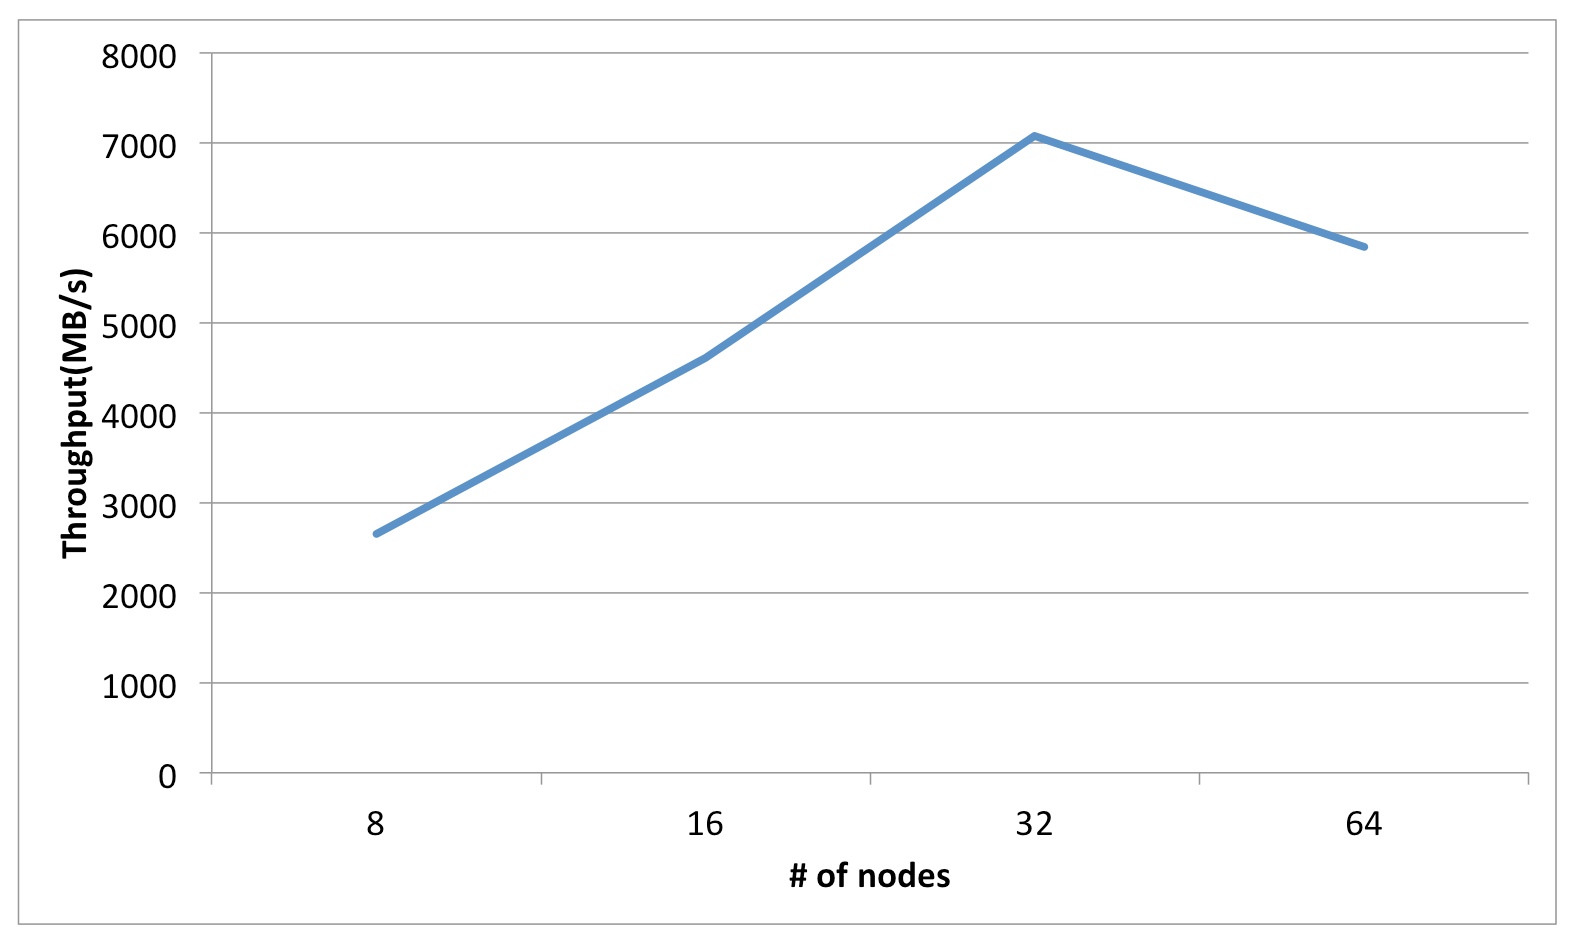
\includegraphics[width=6cm]{throughput_tsubame}
	\caption{I/O Throughput to Lustre inside TSUBAME direct mount}
	\label{throughput TSUBAME}
\end{figure}

\begin{figure}[tb]
	\centering
	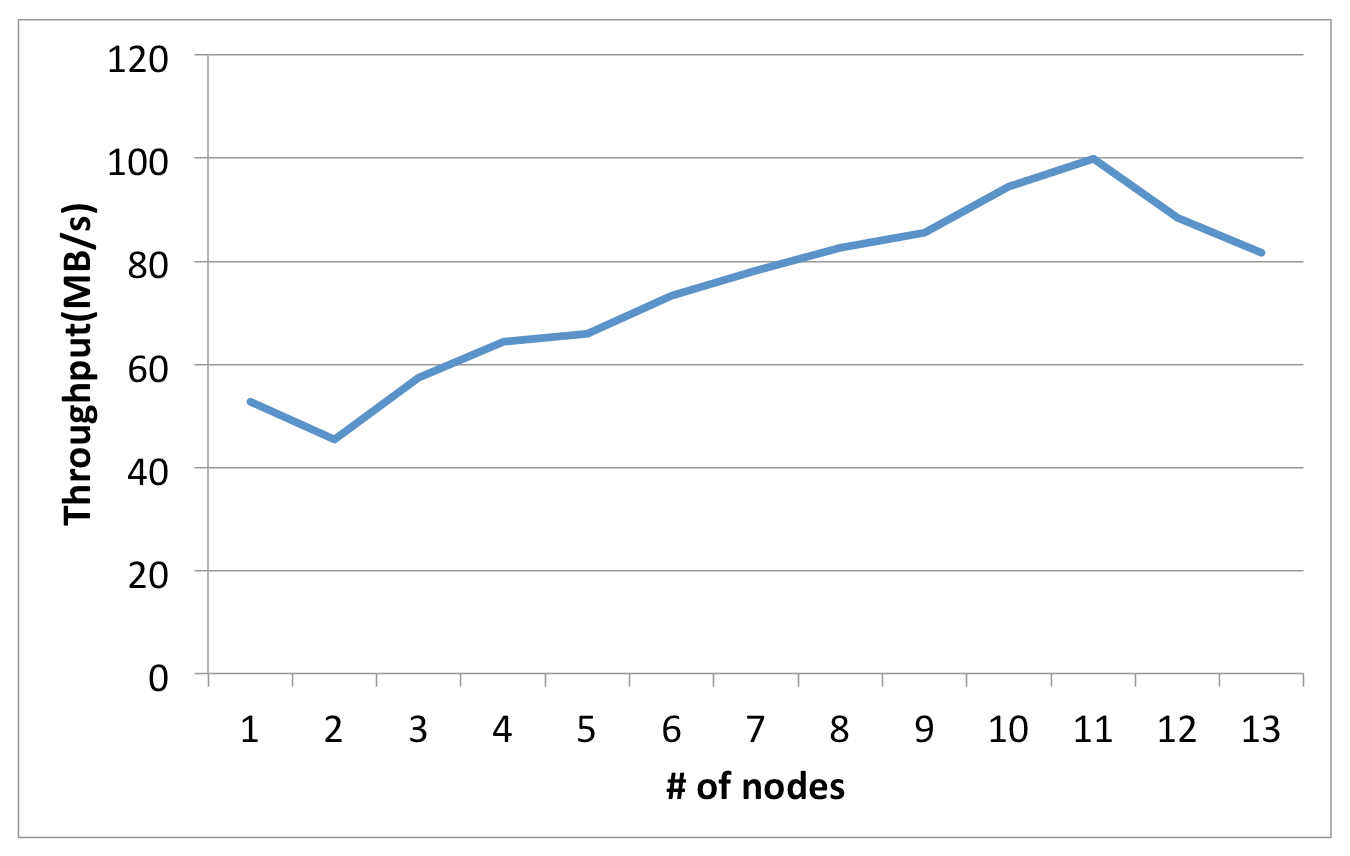
\includegraphics[width=6cm]{AMAZON_to_OUR_LAB}
	\caption{I/O Throughput from AMAZON EC2 to file system inside our lab using sshfs}
	\label{throughput AMAZON to OURLAB}
\end{figure}

\begin{figure}[tb]
	\centering
	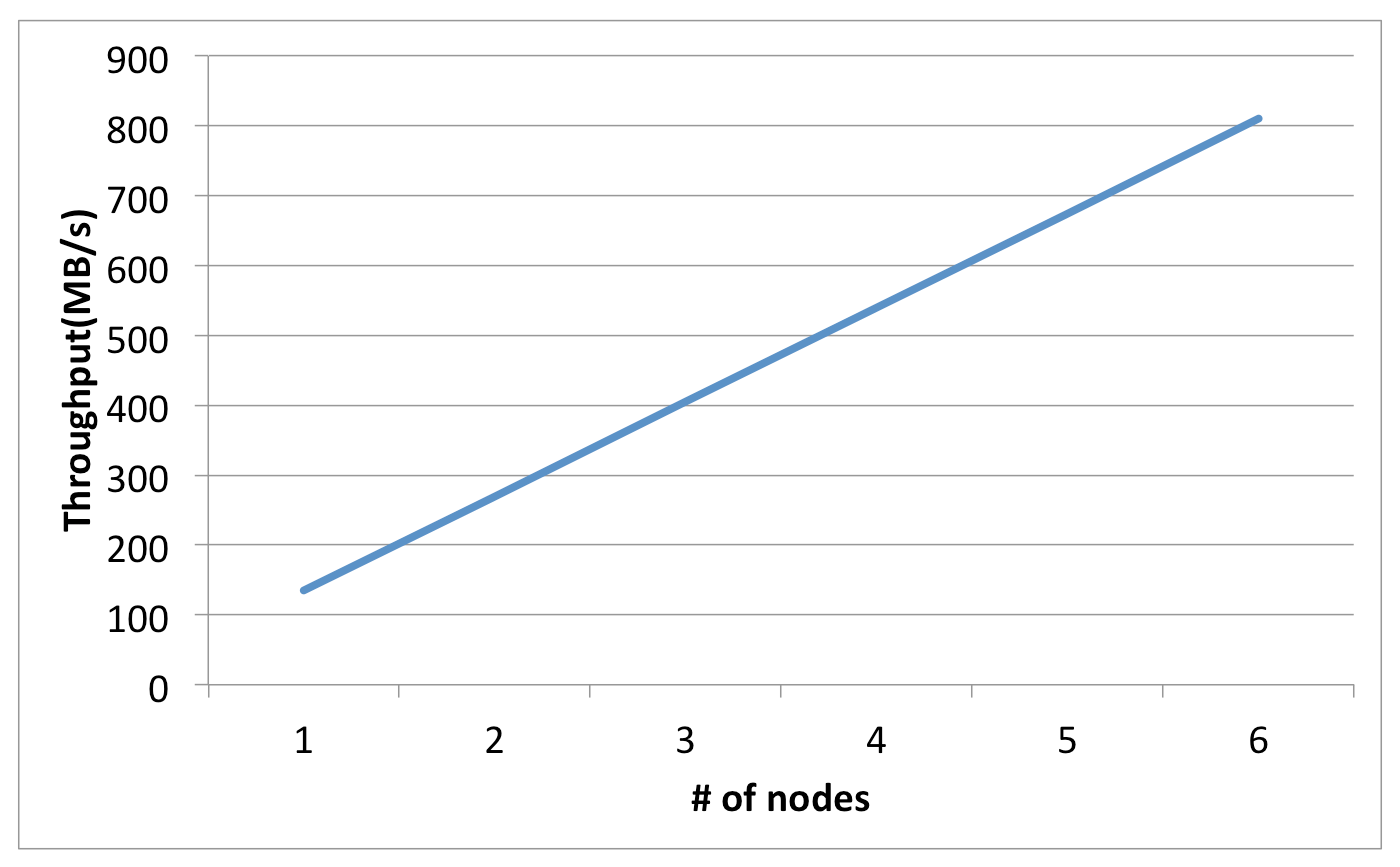
\includegraphics[width=6cm]{point_to_point_AMAZON}
	\caption{point to point connection inside AMAZON}
	\label{point to point connection AMAZON}
\end{figure}

\begin{figure}[tb]
	\centering
	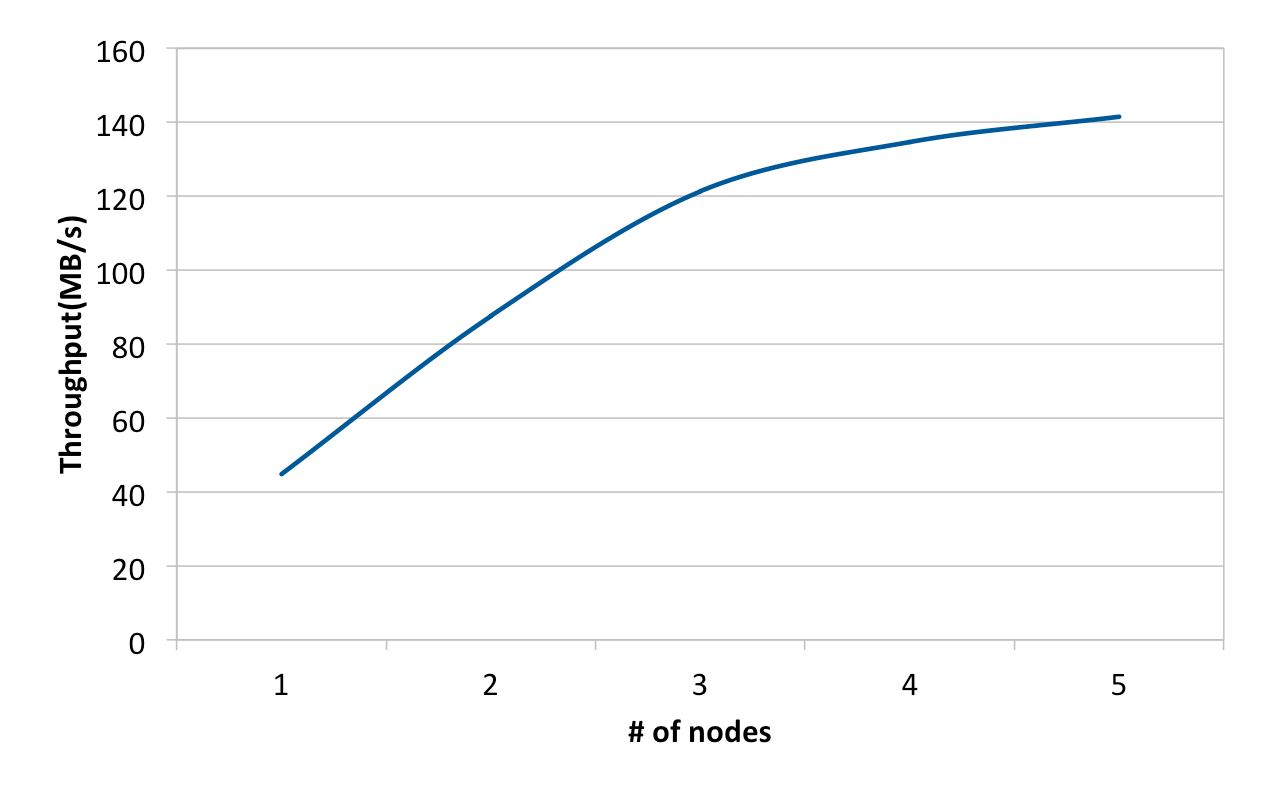
\includegraphics[width=6cm]{point_to_point_lab}
	\caption{point to point connection throughput between AMAZON and our lab}
	\label{point to point connection LAB}
\end{figure}

As we know, throughput gap between interconnection network and Internet is extremely large, also numbers of I/O nodes will affect I/O performance.
We use Iperf\cite{iperf}, which was developed by NLANR/DAST as a modern alternative for measuring TCP and UDP bandwidth performance, and IOR\cite{IOR}, which is widely used for benchmarking parallel file systems using POSIX, MPIIO, or HDF5 interfaces.

Fig.~\ref{throughput TSUBAME} shows I/O throughput between TSUBAME V queue nodes, which run on VM on several shared machines and TSBUAME Lustre file system, which is mounted by using lustre client, it is a interconnection throughput inside TSUBAME supercomputer, we can see that I/O throughput growing as numbers of nodes growing, and the aggregate read and write throughput reach 6-8GB/s with 64 nodes, the same result also can be seen in \cite{checkpointing}.
On the other hand, Fig.~\ref{throughput AMAZON to OURLAB} shows I/O throughput between AMAZON EC2 m3.medium nodes, which have moderate network performance, and a file system machine inside our lab, which has about 1GBit/s Internet access.
Since TSUBAME Lustre can not be accessed outside of TSUBAME because of security problem, instead of TSUBAME Lustre file system, we used a file server inside our lab, which has 1GBit/s internet bandwidth, also because of security problem, we used sshfs\cite{sshfs},which is a filesystem client based on SSH File Transfer Protocol, to mount this file system from AMAZON.
We can see that the I/O throughput also grows as number of nodes grows but the aggregate throughput is only 100-140 MB/s, about 40-80 times smaller than throughput inside TSUBAME.
%From Fig.~\ref{throughput TSUBAME} and Fig.~\ref{throughput AMAZON to TSUBAME Lustre} we can see that the I/O throughput of interconnection inside supercomputer is quit larger than that from AMAZON.
%Also, if we compare the one nodes I/O throughput, 
Also if we compare Fig.~\ref{point to point connection LAB} with Fig.~\ref{throughput AMAZON to OURLAB}, the maximum throughput 
If we move some jobs to AMAZON EC2 with input data stored in TSUBAME Lustre, the execution time will increase because of I/O low throughput,for a data sensitive application, it will be devastating, also according to AMAZON's pay-as-you-go policy\cite{AMAZON_AWS}, longer execution time means more cost.

%But when we compare Fig.~\ref{point to point connection TSUBAME} with FIg.~\ref{point to point connection AMAZON}, the interconnection throughput 
However, if we consider interconnection throughput, as shown in Fig.\ref{point to point connection AMAZON}, although each node can achieve only 1GB/s, the influence between nodes is extremely small, figure shows a perfect linear line also a strong scalability.
Since we can achieve a high interconnection throughput inside a system (HPC system, public cloud), we consider use some nodes as a buffer nodes, using a buffer queue to buffer I/O data and achieve a high throughput.

Although there are some studies about workflow optimization and  balance\cite{Workload}, Since data transfer rate is extremely low in Internet compared with interconnection network and data size processed is extremely large, user do not want to settle their nodes across two systems, so in this model, we just consider the situation that all nodes used for the same job are allocated in the same system.

%3
\section{I/O Bursting Buffer Overview}

%\begin

An overview of I/O burst buffer architecture and two kinds of connection: direct connection and I/O bursting buffer are described in this section.
As we mentioned in the previous section, our model takes advantage of high throughput inside a system, and use buffer queue system in order to increase throughput between two systems.
The main idea is that some of computing nodes serve as a I/O buffer nodes in each system, I/O data will first be buffered in buffer queue in the same system, and then be transferred to final storage system.
%the same computing nodes and then these I/O buffer nodes, after that data will be  transferred to storage in another system.
Two kinds of buffer are used in our I/O burst buffer architecture, the first one is in client computing node, first buffer user I/O in the same node, another one is in I/O buffer nodes.
%Although our goal here is to federate supercomputer with public cloud, since there are a great performance gap between normal supercomputer nodes and public cloud nodes and problem described above, here we consider about federating virtual machine nodes which running on supercomputer physical nodes with public cloud.
%Since public clouds also run virtual machine on physical nodes, in the follow section, we treat the set of supercomputer's virtual machines as a cloud environment, also because only a few public IP address available in each cloud, I/O buffer nodes are required even in direct connection model.


%Reading operation describes operations when issues reading data from another cloud storage, and writing operation describes operation when issues writing data to another cloud storage

%Migration operation occurs when some nodes have to be shut down in one cloud 
%all jobs running on these nodes have to be backed up by using snapshot, 

\subsection{System Environment}
First a general system used in following sections is defined as follow:

%For security consideration and the fact that IPv4 addresses becomes rare,
\begin{itemize}
	\item All computing nodes are connected by large bandwidth and interconnection network, note network topology maybe different in each system, so topology is not specified here, interconnection network performance is measured by throughput.
	\item There are a constant number of public IP addresses can be assigned to some computing nodes.
	\item There is a shared storage for date sharing inside system, all computing nodes are connected with shared storage, also the filesystem of shared storage is not specified and performance is measured by throughput.
\end{itemize}

\subsection{I/O Burst Buffer Architecture}

\begin{figure}[tb]
	\centering
	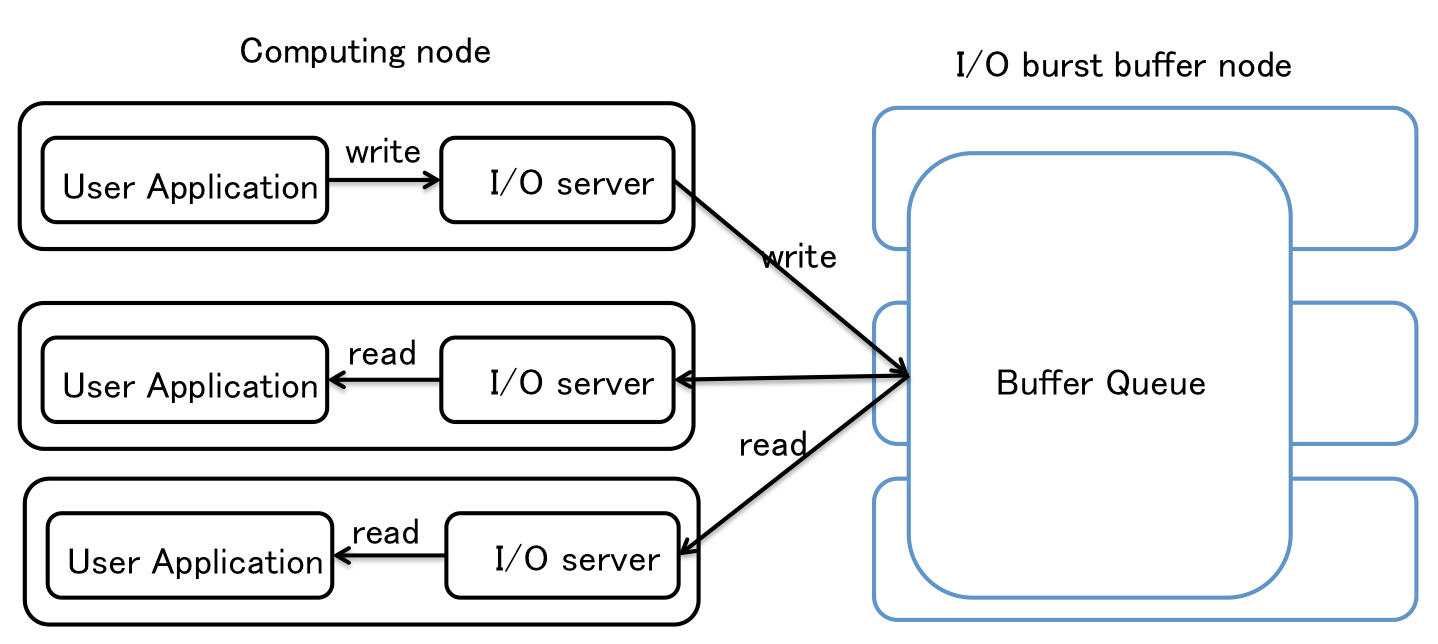
\includegraphics[width=6cm]{IOserver}
	\caption{I/O server and buffer queue}
	\label{I/O server}
\end{figure}

\begin{figure}[tb]
	\centering
	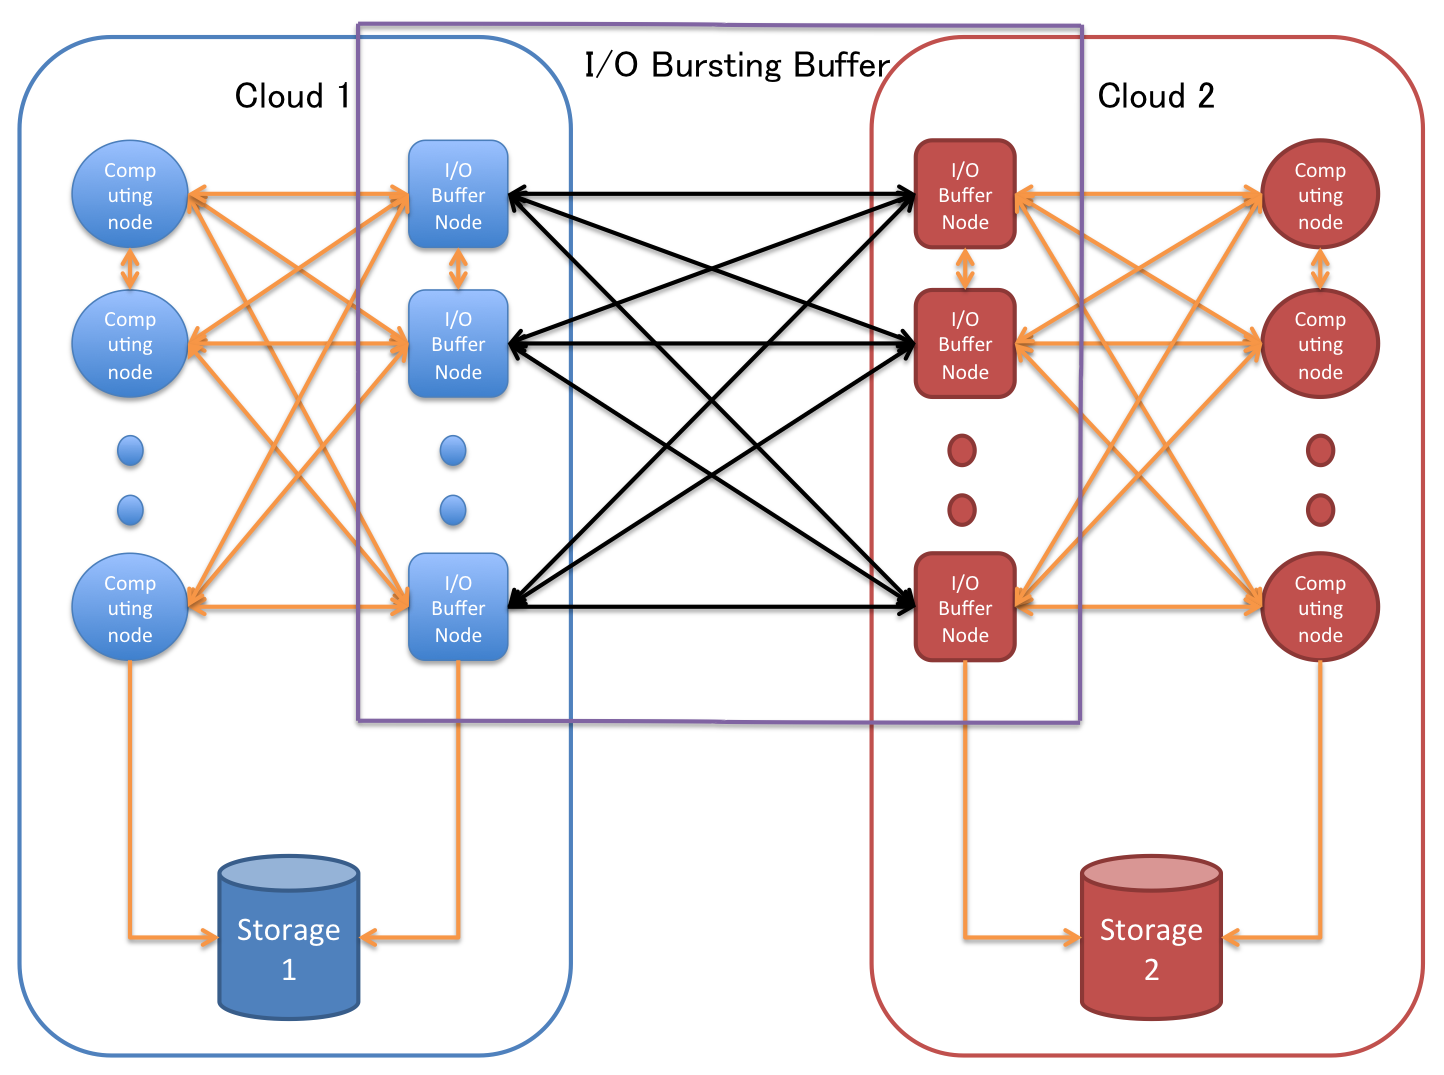
\includegraphics[width=6cm]{overview}
	\caption{overall illustrate of I/O Burst Buffer Architecture}
	\label{overview}
\end{figure}

%Fig.~\ref{overview} and Fig.~\ref{I/O server} are the overall illustrate of I/O Bursting Buffer:
There are two kinds of nodes in our I/O burst buffer architecture: \emph{computing nodes} and \emph{I/O burst buffer nodes}, computing nodes run user's application,which assigned only  and I/O burst buffer nodes, which assigned both private IP address.

Fig.~\ref{I/O server} is a illustrate of I/O server inside client nodes and buffer queue in I/O burst buffer nodes.
In each computing node, there is a I/O server, which is a filesystem client used to buffer I/O data and send to or read from I/O buffer nodes.
Among I/O burst buffer nodes, there is a master nodes, which maintain a global buffer queue and a namespace, controll buffer read and write, and manage I/O buffer nodes, buffer data is distributed to all I/O buffer nodes in order to enable concurrent read and write.

When a user application issue a write request, I/O data will be buffered in that node by I/O server, when user close the file, call flush function or I/O data size exceed I/O server buffer size, I/O data will be transferred to I/O burst buffer.
First, I/O server sends the size of I/O data to master I/O burst buffer node, master node return a list of several I/O buffer nodes, then I/O server split I/O data into pieces, and sends each pieces to a I/O buffer node, after data transfer finished, that file will be added to buffer queue and namespace, and this file can be seen by all computing nodes, since we assume that all nodes used by the same job are allocated in the same system, so data consistency can be guaranteed since that.
Buffer queue operation including data write back and operation when queue is full will be described in following section.

When user issue a read request, there are two conditions: file is buffered in buffer queue in I/O burst buffer, or file is stored only in storage in another system.
In the first cases, file can be transferred to computing nodes from buffer queue directly, and can achieve a high throughput.
If data is not in buffer queue, then a read operation described below will be executed, since data must be transferred from storage in another system, in this case, throughput will depend on Internet condition and it is hard to achieve a high throughput.

Fig.~\ref{overview} shows a overall illustrate of I/O burst buffer architecture.

%Consider there are two systems, named system 1 and system 2


%Arrows stand for network connection.
%Orange arrows are interconnection networks inside cloud, although two clouds used the same color for interconnection networks, bandwidth can be different, also the topolopies are not specified and can be different in each cloud.
%Black arrows are Internet connections, since there are a few amount of public IP addresses available, only I/O buffer nodes are connect to Internet, also the amount of available public IP address becomes the upper bound of the amount of I/O buffer nodes in each cloud. 
%Although nodes with private IP address can use route or other net device to connect to Internet, but consider about security problem, also using route will reduce concurrent data transfer rate, here we assume all nodes in cloud only connect to local private network except I/O buffer nodes which connect to both local network and Internet.

%Circles stand for computing nodes, which are used for standard computation.
%Here we assume all computing nodes can communicate with each other, and also I/O buffer nodes and shared storage in the same cloud environment.
%Squares are I/O buffer nodes, these nodes are used for data transfer between clouds, and are assigned with both public and private IP addresses.
%I/O buffer nodes can use the same machine or VM as computing nodes, or can use network optimized nodes for larger throughput, but it is not required here.
%Cylinders are shared storages, which are used to store data used by computing nodes, usually shared storage is consist of several nodes with a distributed filesystem and uses a better network, offers a large throughput.

%Since there is a big gap between cloud inside data transferring and accross two clouds in throughput, our goal is to fill the gap. 

%For convenience, in the following section we assume data is stored in Cloud 1's shared storage, and computing nodes in Cloud 2 are used for computation. 

%in this subsection, we introduce operations of buffer queue write back.

\subsection{Read and Write}

\begin{figure}[tb]
	\centering
	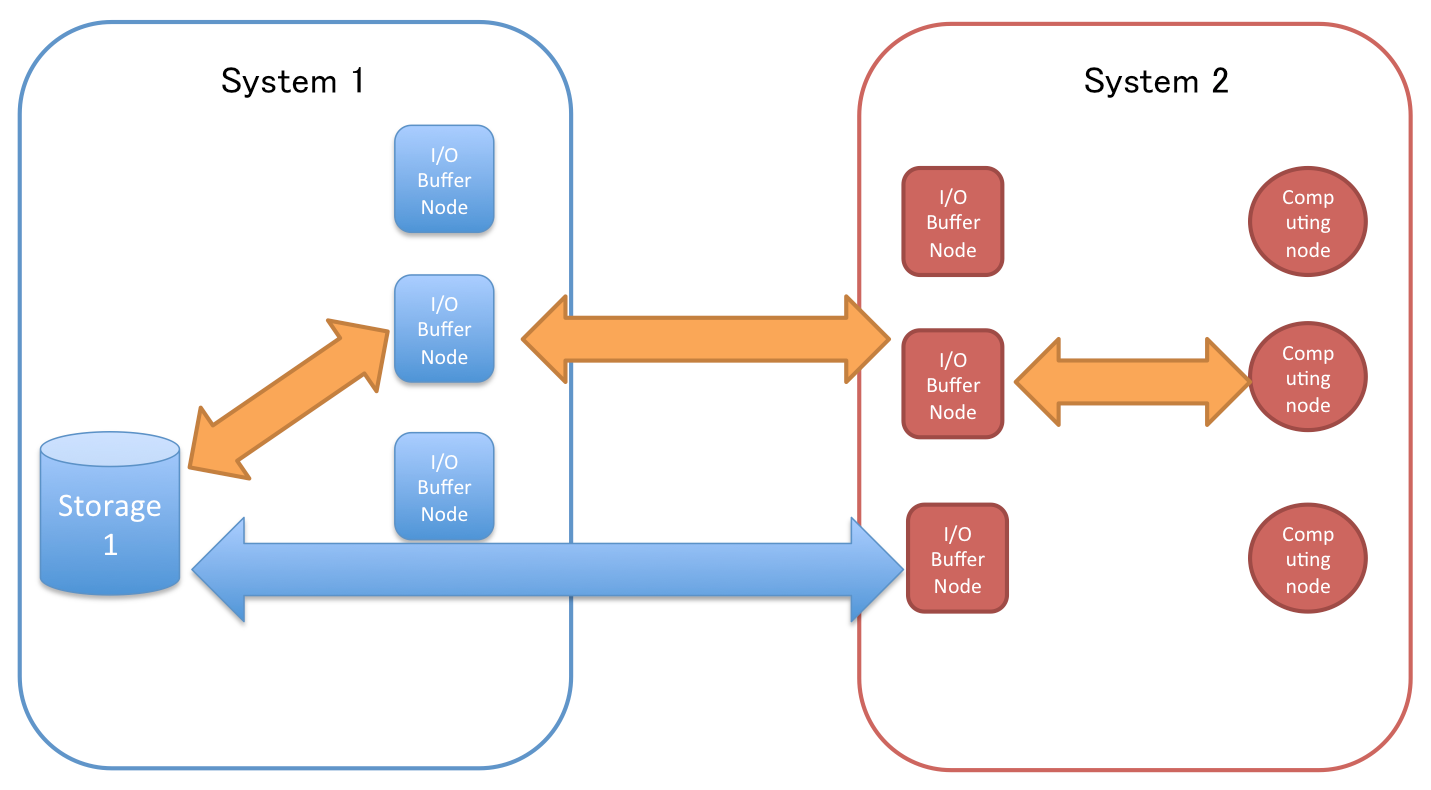
\includegraphics[width=6cm]{read_and_write}
	\caption{read and write operation}
	\label{read and write}
\end{figure}

In this section we describe operations when file is not in I/O buffer nodes or file needs to be write back to storage in another system.
We propose two kinds of model: one-side buffer and two-side buffer.

\subsubsection{One-side Buffer}

As Fig.~\ref{read and write} blue arrow shows, one-side buffer is a connection between I/O buffer nodes in system 2 and storage in system 1 directly.
When I/O nodes need to write data back to storage in another system, since data is already spread among I/O nodes, a parallel write can be achieve to fully utilize the Internet bandwidth.

Similarly, when I/O nodes need to read data from storage in another system, several I/O nodes will be assigned equal size of data, and then these nodes read assigned piece of data from the storage concurrently.

There will be two problems in this solution:
\begin{itemize}
	\item First storage should be opened to Internet, in order that I/O nodes can read from or write to it.
		However storage system in supercomputer store Petabyte of research data, open the access of storage system means that put these research data under risk of attack.
	\item As we mentioned before, throughput of one side communication is lower than two side communication, since we use SSH protocol based File system for security reason.
		also two side communication can achieve a higher throughput with fewer nodes, according to pay-as-you-go policy, reduce number of nodes can reduce cost.
\end{itemize}
%data firstly be splitted into number of I/O buffer nodes in cloud 2 pieces and assign one I/O buffer node one piece, then I/O buffer nodes start reading assigned data concurrently in order to fully utilize Internet bandwidth.
%After reading finished, I/O buffer nodes send data to each computing node Simultaneously, there data will be restructure by using protocol described below.

%Like reading, when computing nodes start to output data, first data will be buffered inside that nodes.
%After output finished, data will be splitted into number of I/O buffer nodes in cloud 2 pieces, and assign one I/O node one piece, then data will be sent to all I/O buffer nodes concurrently.
%When I/O buffer nodes received data, then they writing data back to storage in cloud 1.

\subsubsection{Two-side Buffer}

On the contrary, two-side buffer solution use I/O buffer nodes in both two systems as Fig.~\ref{read and write} orange arrows show.
I/O data will be split twice, transferred throughput two sides of I/O buffer nodes and then reached the destination.

Consider I/O nodes in system 2 issue a write back operation, also, data is already spread among I/O nodes in system 2, each I/O node will find a pair among I/O nodes in system 1, then transfer their piece of data to system 1 concurrently.
After I/O node in system 1 received data, they write data back to storage in system 1.

Compared with one-side buffer, two-side buffer required one more data transfer (I/O nodes to storage in the same system), if storage data transfer throuhput become a bottleneck, two-side buffer will cost more time than one-side buffer.
Also, two-side buffer require both systems allocate I/O buffer nodes, if node usage is charge in both system, total cost may be larger than one-side buffer.

%the bottleneck is still Internet throughput, since interconnection is far faster than Internet.
Since two-side buffer does not read data from or write data to storage directly, it means we can compress data before transfer it, though it will take some time to compress and decompress data, when the Internet throughput is extremely low, compress and decompress time will be far smaller than tranferring time, and compress data can make more data buffered in buffer queue.
Also, unlike one-side buffer, two-side buffer do not require storage to be opened to Internet, only required several I/O nodes have access to Internet.

%I/O bursting buffer model may be used when throughput of direct connection between I/O buffer nodes and storage in different cloud is smaller then throughput between I/O buffer nodes, it is possible when storage is consist of few nodes, and direct connection will be 1-N connection, on the contrary, connection between I/O buffer nodes is N-N connection, has larger parallelism.

%When computing nodes issue read request, first we check whether the file has been cached in I/O buffer nodes in cloud 1, if not, File will be splitted into the same number of I/O buffer nodes in cloud 1, and each I/O buffer node will be assigned a piece of split, then all I/O buffer nodes start reading assigned piece of data from shared storage simultaneously to fully utilize the bandwidth.% I/O buffer nodes use a main index to refer to the data position in global data.

%After transferring data from shared storage finished, I/O buffer nodes in cloud 1 will connect with all I/O buffer nodes in cloud 2, then split data piece and into number of I/O buffer nodes in cloud 2,
%here a sub-index is used to refer to each piece's position, 
%then transfer these pieces to I/O buffer nodes in cloud 2 concurrently in order to fully utilize Internet bandwidth.

%When data transfer finished, I/O buffer nodes connect with all computation nodes which needs data, then transfer data to the corresponding position by using a index protocol described below, of cause all data transfer are done in parallel.

%Data writing operation doing the opposite operation as reading operation.
%When a computing node in cloud 2 issues data writing, output data will be first buffered by I/O server in that node.
%After output finished, I/O server connects with all I/O buffer nodes in the same cloud, and split output data into the number of I/O buffer nodes, then send each piece of data to each I/O buffer nodes Simultaneously.

%I/O buffer nodes then again split data into the number of I/O buffer nodes in cloud 1, like reading operation, here sub-index is used to refer to data position. and then start to transfer data concurrently. 

%Then I/O buffer nodes write data to storage in cloud 1.



\begin{comment}
\subsubsection{Index Protocol}

\begin{figure}[tb]
	\centering
%	\includegraphics
	\caption{index protocol}
	\label{index protocol}
\end{figure}

As Fig.~\ref{index protocol} shows, two indexs are used in this protocol: main index and sub-index.
There are two phases of data splitting in both reading and writing operation, 
\end{comment}
%\subsubsection{Node Migration}
%Node migration happens when some nodes have to be shut down due to some situation like power problem in summer, and still need to provide service to users.
%In these cases, nodes will be migrate by snapshot, usually snapshots of these nodes will first be stored into shared storage, then these snapshots will be transferred to another cloud, and start VM by using these snapshots.

%However, the low throughput between direct connection of nodes and storage in different environment will still be a bottleneck for quick migration.
%When using I/O buffer nodes 

\section{I/O Burst Buffer Model}

%\begin{figure}[tb]
%	\centering
%	\includegraphics
%	\caption{definition}
%	\label{definition}
%\end{figure}

Throughput-based Model, Cost-based Model and buffer queue write back model will be described in this section.
Throughput-based Model compare one-side buffer throughput with two-side buffer, cost-based model compare one-side buffer cost with two-side buffer, and buffer queue write back model. 
We make definitions shows in Table.~\ref{definition} in order to describe our model:
\begin{table}[tb]
	\caption{Definition of parameters}
	\label{definition}
\begin{tabular}{|p{3cm}|p{5cm}|}
	\hline
	$c_1,c_2$&Numbers of computing nodes in system 1 and system 2\\\hline
	$n_1, n_2$&Numbers of I/O buffer nodes in system 1 and system 2.\\\hline
	$m_1,m_2$&Available memory size for each I/O node in system 1 and 2, also the maximum buffer size will be $n_1\times m_1$ and $n_2\times m_2$\\\hline
	$D_1(n_2),D_2(n_2)$&Throughput when $n_2$($n_1$) I/O nodes in system 1 (system 2) connect to storage in the other system directly, here we assume only I/O nodes in each system have Internet connection.\\\hline
	$I(n_1,n_2)$& 	Internet throughput using $n_1,n_2$ I/O buffer nodes respectively, Since overall Internet throughput is affected by number of nodes involved in connection.\\\hline
	$E_1(n_1), E_2(n_2)$&Interconnection network throughput in system 1 and 2, although interconnection throughput is also affected by numbers of I/O nodes and computing nodes, numbers of users will running application on different number of computing nodes.\\\hline
	%, it is difficult to compute each throughput, so here we use $E_1(n_1)$ to refer to limitation of maximum throughput of interconnection network in system 1 with $n_1$ I/O nodes, likely ,$E_2(n_2)$ is limitation of maximum throughput of interconnection network in system 2 with $n_2$ I/O nodes.
	$M_1(n_1),M_2(n_2)$& Throughput of connection between storage and $n_1$ I/O nodes in system 1 and storage and $n_2$ I/O nodes in system 2.\\\hline
	$C_1\_Money(T)$,$C_2\_Money(T)$& Cost for standard node in system 1 and 2 for $T$ time usage\\\hline
	%and cost for node in system 1 is $C_2\_Money(T)$ for $T$ time usage, and since I/O nodes may use a better network, 
	$C_1\_High\_Money(T)$,$C_2\_High\_Money(T)$& cost I/O nodes in system 1 and 2 for $T$ time usage, since I/O nodes may use a better network condition, we assume it will cost more than normal nodes.\\\hline
\end{tabular}
\end{table}

\subsection{Throughput-based Model}
%There are many facts will affect throughput of Internet, so here a moniter is used to evaluate throughput between 
In the case of one-side buffer, there are two data transfers: computation nodes to I/O buffer nodes in system 2, I/O buffer nodes in system 2 to storage in system 1, so throughput will be:
\begin{equation}
	\text{throughput}_{\text{one-side}}=\min\{D_1(n_2),E_2(n_2)\} \label{throughput1}
\end{equation}

In the case of two-side buffer, there are three data transfers: computation nodes to I/O buffer nodes in system 2, I/O buffer nodes in system 2 to I/O buffer nodes in system 1, I/O buffer nodes in system 1 to storage in system 1, throughput will be:

\begin{equation}
	\text{throughput}_{\text{two-side}}=\min\{M_1(n_1),I(n_1,n_2),E_2(n_2)\} \label{throughput2}
\end{equation}

In this throughput-based model, these two throughputs are evaluated, and a switch is based on these two values:

\begin{equation}
	\begin{cases}
		\text{throughput}_{\text{one-side}} \geq \text{throughput}_{\text{two-side}} & \text{use one-side}\\
		\text{throughput}_{\text{one-side}} < \text{throughput}_{\text{two-side}} & \text{use two-side}
	\end{cases}
\end{equation}

\subsection{Cost-based Model}
In the case of cost-based model, we consider
using \ref{throughput1},and \ref{throughput2} total time for transferring unit size of data can be compute as:

\begin{equation}
	\begin{cases}
		T_1=\frac{1}{\min\{D_1(n_2),E_2(n_2)\}} & \text{one-side}\\
		T_2=\frac{1}{\min\{M_1(n_1),I(n_1,n_2),E_2(n_2)\}} &\text{two-side}
	\end{cases}
\end{equation}

here we compute cost by using $T_1,T_2$:
\begin{equation}
	\text{cost}_\text{one-side}=c_2\times C_2\_Money(T_1)+n_2\times C_2\_High\_Money(T_1)
\end{equation}
\begin{align}
	\text{cost}_\text{two-side}&=c_2\times C_2\_Money(T_2)\\\nonumber 
				     &+n_1\times C_1\_High\_Money(T_2)\\ \nonumber
				     &+n_2\times C_2\_High\_Money(T_2)
\end{align}

In this throughput-based model, these two throughput are evaluated, and a switch is based on these two values:

\begin{equation}
	\begin{cases}
		\text{cost}_{\text{one-side}} \geq \text{cost}_{\text{two-side}} & \text{use one-side}\\
		\text{cost}_{\text{one-side}} < \text{cost}_{\text{two-side}} & \text{use two-side}
	\end{cases}
\end{equation}

%\subsection{}
%\subsection{Migration Model}
%Since there are some condition that some supercomputer nodes must be shut down, and jobs running on these nodes have to be migrate to another cloud. There are 
%\begin{equation}
%	Data	
%\end{equation}
\subsection{Buffer Queue Write Back Model}

\begin{figure}[tb]
	\centering
	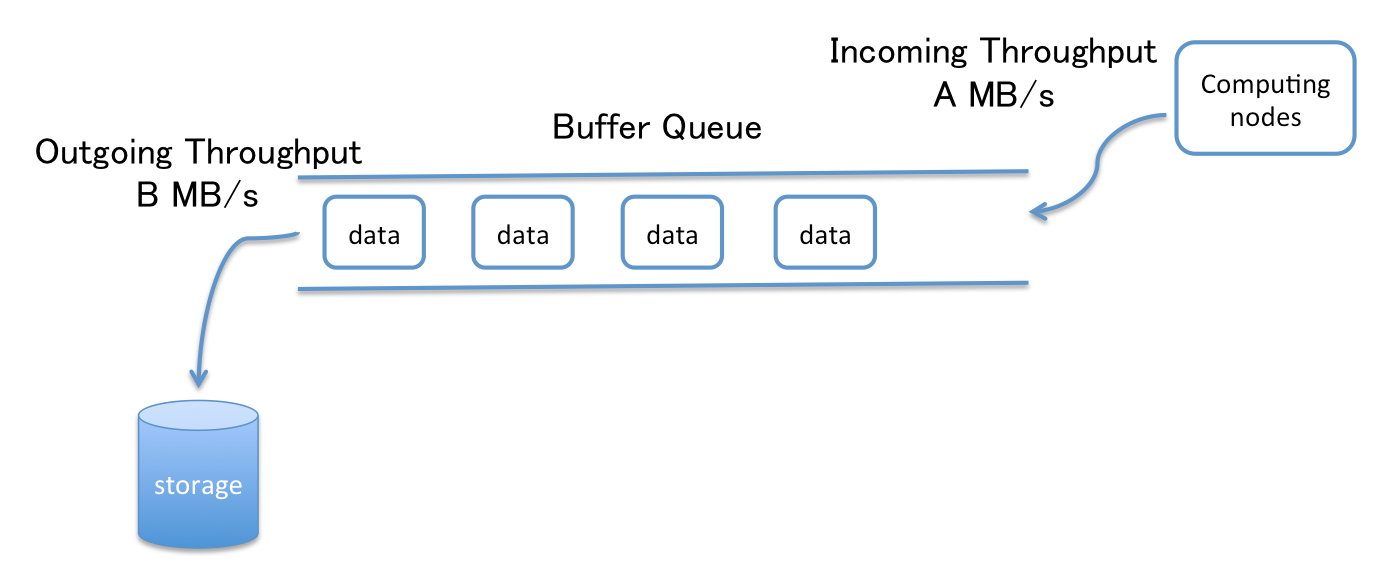
\includegraphics[width=6cm]{buffer_queue}
	\caption{buffer queue}
	\label{buffer queue}
\end{figure}

If the buffer size is unlimited. then we can buffer all data in the I/O buffer nodes, and achieve a high throughput in cloud burst.
However buffer size can not be unlimited, we can not buffer all data in the I/O buffer nodes, data in buffer nodes have to be write back to storage in another system.
The problem is which data should be written back to storage, like cache in cpu, if we can reduce cache miss in this situation, we can increase throughput. 
According to data locality, we use a priority queue to determine which data should be write back.

Consider Fig.~\ref{buffer queue}, assume average incoming throughput is A MB/s and average outgoing throughput is B MB/s, if A always larger than B, after $T$ time buffer queue will full.
\[T=\frac{m_2\times n_2}{A-B}\]

After that, since buffer queue is full, I/O server can not send more data to I/O buffer nodes, have to block any read and write request since that.
In this case, jobs running on public cloud have to be moved back to original system until buffer queue is empty.

\section{Evaluation}

\begin{figure}[tb]
	\centering
	%\includegraphics[width=6cm]{}
	\caption{throughput comparison with and without I/O burst buffer}
	\label{throughput}
\end{figure}

\begin{figure}[tb]
	\centering
	%\includegraphics[width=6cm]{}
	\caption{cost comparison with and without I/O burst buffer}
	\label{cost}
\end{figure}

\begin{figure}[tb]
	\centering
	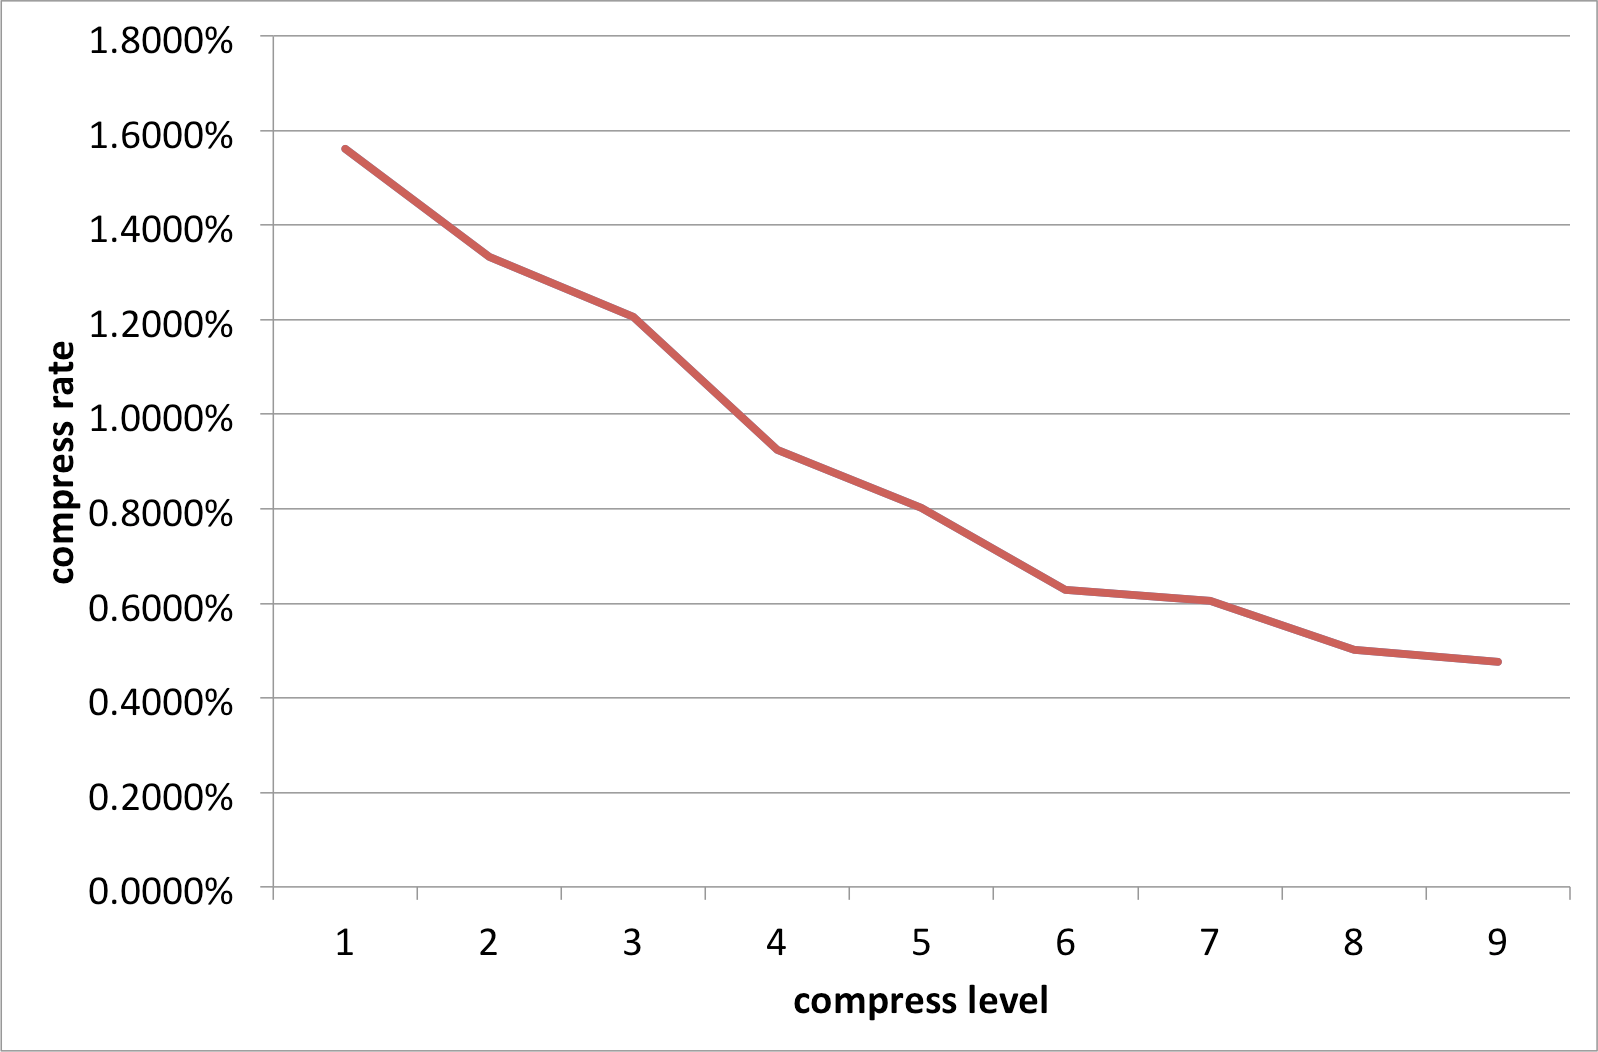
\includegraphics[width=6cm]{compress_rate}
	\caption{compress rate}
	\label{compress rate}
\end{figure}

\begin{figure}[tb]
	\centering
	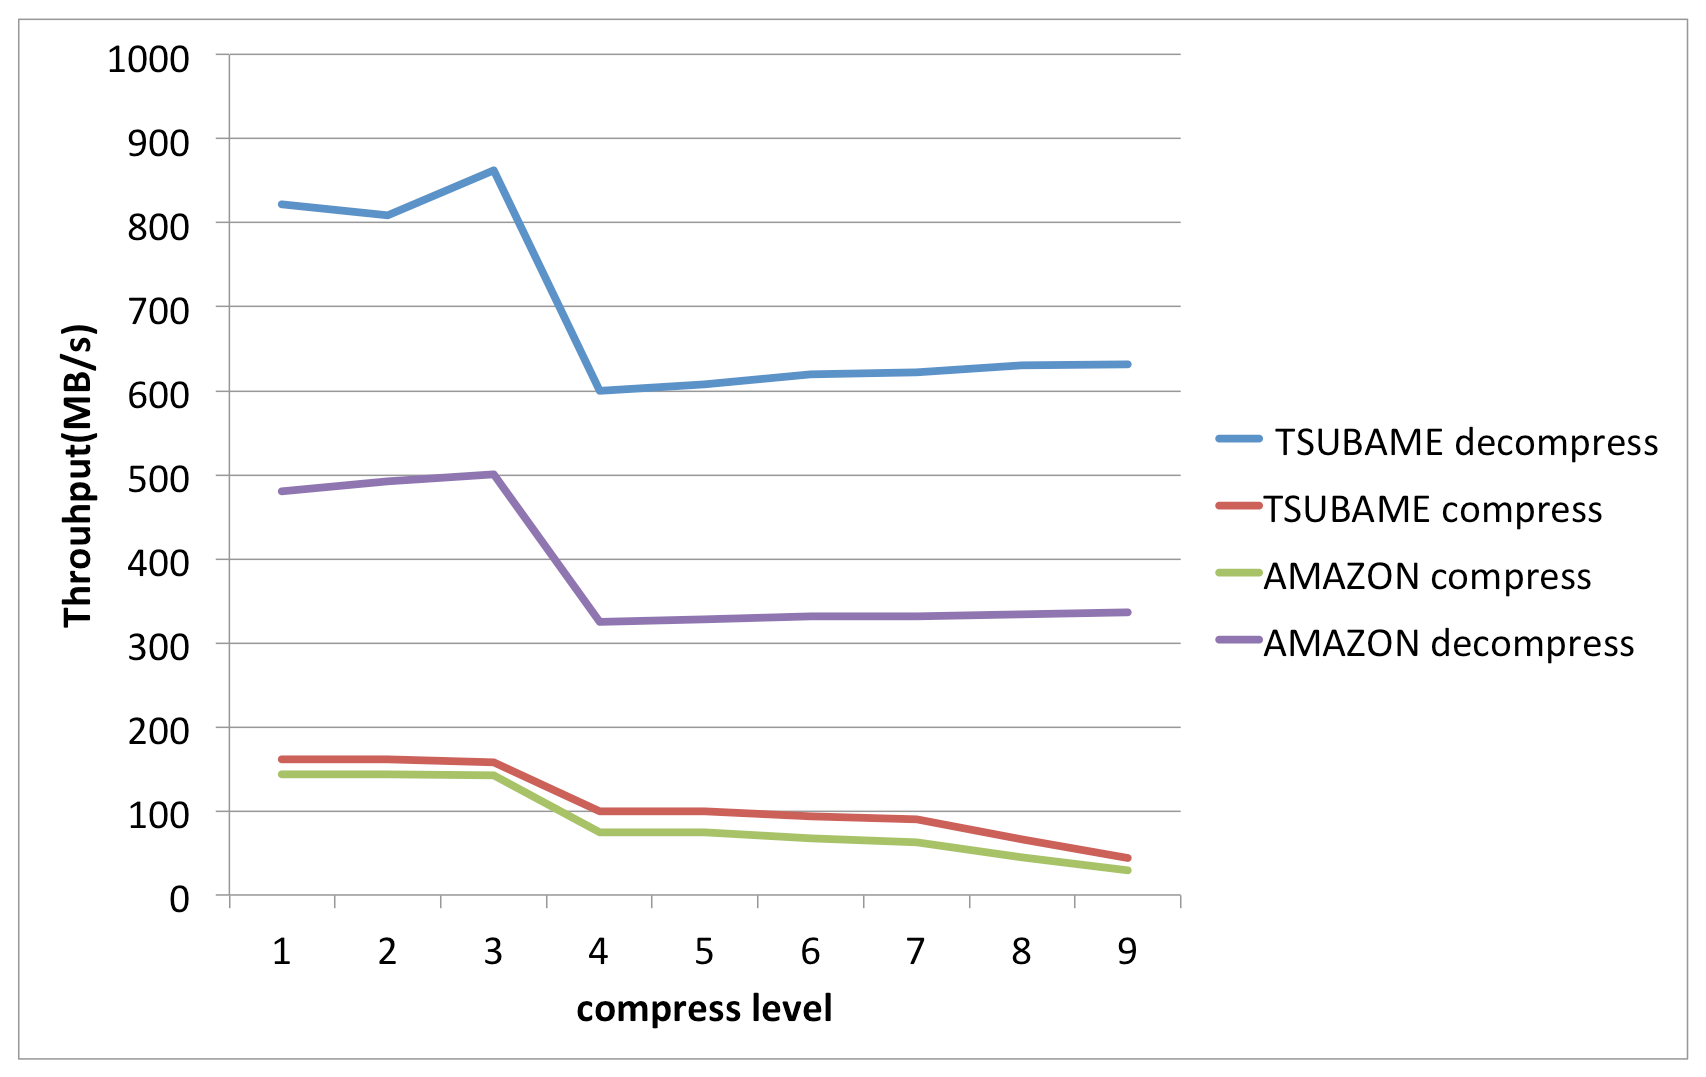
\includegraphics[width=6cm]{compress_time}
	\caption{compress time on TSUBAME V queue and AMAZON EC2}
	\label{compress time}
\end{figure}

\begin{figure}[tb]
	\centering
	%\includegraphics[width=6cm]{}
	\caption{throughput comparison with and without compress}
	\label{compress}
\end{figure}

\begin{figure}[tb]
	\centering
	%\includegraphics
	\caption{cache hit and miss throughput comparison}
	\label{cache hit}
\end{figure}

%\begin{figure}[tb]
%	\centering
%	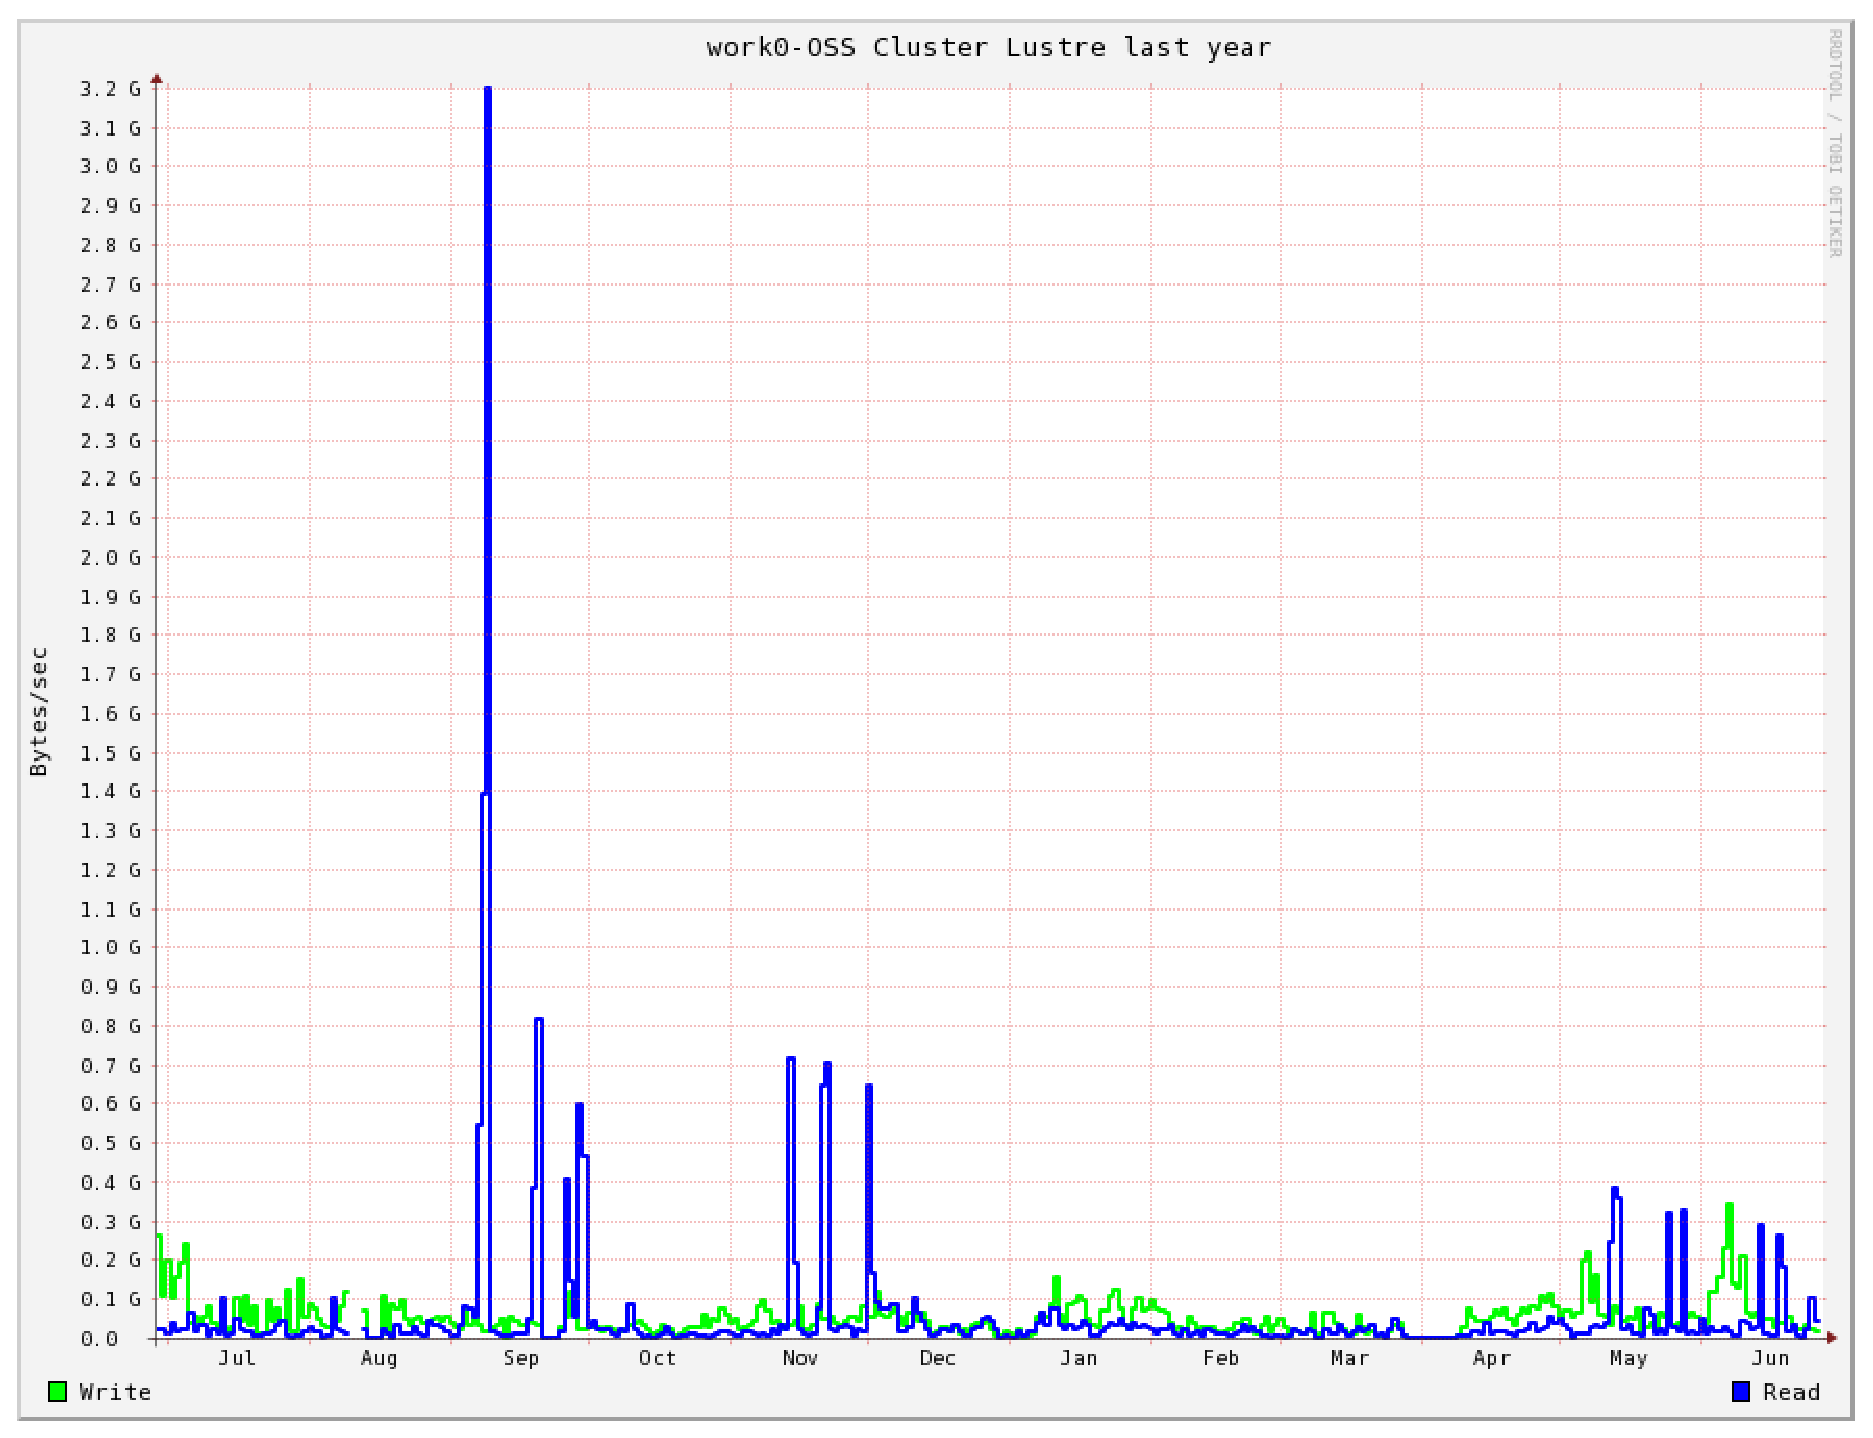
\includegraphics[width=6cm]{tsubamelustre}
%	\caption{TSUBAME Lustre workload}
%	\label{Lustre workload}
%\end{figure}

In this section, a simulation will be introduced based on data taking from several benchmarks on both TSUBAME V queue and AMAZON EC2 public cloud Tokyo region, using
%m3.medium instance, which has a moderate Ethernet condition and one vcpu with 3.75GiB memory, and
m3.xlarge instance, which has a high Ethernet condition and 8 vCPUs with 30GiB memory, run Amazon Linux AMI 2014.03.2(HVM) ( Fig.~\ref{throughput TSUBAME}, Fig.~\ref{throughput AMAZON to OURLAB}. Fig.~\ref{point to point connection AMAZON}, Fig.~\ref{point to point connection LAB} ).
%According to these data and definition described above, we use values defined below.

%\begin{center}
%\begin{tabular}[tb]{|c|c|}\hline
%	$D_2$&$E_1$\\\hline
%	8TB/s&1.08Gbit/s(135MB/s)\\\hline
	
%\end{tabular}
%\end{center}
For throughput between two systems and inside system, from benchmark data, it shows it is hard to achieve a high throughput with only one nodes, and also there is a limit on maximum throughput between two systems and inside system.
Although incresing nodes can increse throughput before reach the maximum, throughput achieved by each nodes decrease because of conflict.
For these reason, we use following formular for throughput between two systems and inside system.
%TSUBAME and AMAZON EC2, we use similar model in \cite{ccgrid}:
\begin{equation}
throughput=-Ax^2+Bx+C~~ A,B>0\\
\end{equation}
we use following equations to determine $A,B,C$
\begin{equation}
\begin{cases}
	-A+B+C=throughput_{one}\\\nonumber
	\frac{B}{2A}=n_{max}\\\nonumber
	-An_{max}^2+Bn_{max}+C=throughput_{max}\\
\end{cases}
\end{equation}

First, we compare throughput with and without I/O buffer nodes.
Since it is hard for one node to fully utilize Internet and Ethernet bandwidth, according to Fig.~\ref{throughput AMAZON to OURLAB}, we assume that one node can achieve half of maximum bandwidth.
We can see from Fig.~\ref{throughput}, when interconnection throughput is larger than Internet throughput, our I/O buffer can achieve a higher throughput.

Then, we compare overall cost by using I/O burst buffer, 

we compare throughput with and without compression, Fig.~\ref{compress rate} shows compress and Fig.~\ref{compress time} shows compress and decompress time on TSUBAME V queue and AMAZON EC2 with a different compress level by using zlib\cite{zlib}.
We can achieve a high compress rate, but the throughput is low, up to 160MB/s, depends on compress level, it is hard to find a compress library can compress data faster and smaller, so the compress throughput may become a bottleneck.
On the other hand, the compress rate is high, since the buffer size is limited, if we can make data smaller, it means we can increase the buffer hit rate, Fig.~\ref{cache hit} shows a throughput comparison between cache miss and hit.

Fig.~\ref{compress}
\section{Conclusion and Future Work}

In this paper, we propose a I/O burst buffer architecture to burst I/O throughput, provide throughput-based, cost-based and queue write back model, and provide a simulation based on several benchmarks on TSUBAME supercomputer and AMAZON EC2 public cloud.
we use several nodes in each system as a I/O buffer nodes, and use data buffering to hide the low throughput between two systems connected by Internet.

From simulation result, we showed that our I/O burst buffer can increase I/O throughput when Internet throughput is far smaller than interconnection throughput as well as reducing the overall cost.

For future work, we plan to implement this I/O burst buffer architecture.
\bibliography{reference}
\end{document}
